\chapter{Specialising and optimising xDSL pattern rewriting}
\label{chap:specialising-optimising-pattern-rewriting}

%% Introduction and goals (make faster and only constrained by language runtime)
% Hook
In \autoref{chap:measuring-compiler-performance}, we constructed a set of experiments to empirically compare the current performance of the xDSL and \ac{mlir} compiler frameworks.
% Argument
Our overall aim is to use these experiments to contrast the performance of static and dynamic languages for the implementation of user-extensible compiler frameworks, using \ac{mlir} and xDSL as proxies for these two categories respectively.
However, the experiments so far measure a combination of the effects of dynamism in the language runtime and implementation details of the framework, with the former obscuring our measurements of the latter.
% Link
In order to use the frameworks for our aims, our measurements must be as independent of implementation details as possible.

% Hook
In this chapter, we disentangle these effects by specialising the xDSL framework to implement only a single workload.
% Argument
To do this, we manually identify and remove computation performed by the framework which is unnecessary to its execution of this workload. For example, the framework may calculate and check values that are known as runtime invariants for the selected workload. Checking properties of empty fields is one such example. Since this checking does not contribute to the workload's behaviour, it can be removed. Another example is functionality which improves the expressivity of the framework's API, such as runtime type checks to support polymorphism of arguments. Since the workload only uses a single facet of this API, this can also be removed.
% One common example of this is functionality which improves the expressivity of the framework, such as runtime type checks to support polymorphism of arguments. A second example is calculating and checking values which are known as runtime invariants for the selected workload, such as checking properties of empty fields.
% In this process, we manually identify and remove computation performed by the framework which is unnecessary to its execution of this workload. This computation broadly falls into two categories. The first is functionality which improves the expressivity of the framework, such as runtime type checks to support polymorphism of arguments. The second is calculating and checking values which are known as runtime invariants for the selected workload. % DONE: Does it make sense to split these into categories, almost the same thing in some sense -- no!
By eliminating the performance overheads from these unnecessary computations, we reach an implementation representative of the best-case performance of Python for this workload.
% Link
The benefits of this specialisation are twofold. Firstly it reveals inefficiencies in xDSL which can be optimised to improve the general performance of the framework. Secondly, it provides a true performance baseline for dynamic languages irrespective of implementation details which can be used to quantify the impact of dynamism in \autoref{chap:dynamism-pattern-rewriting}.


\section{Micro-benchmarks}
\label{sec:specialising-ubenchmarks}

%% Link back to micro-benchmarks and summarise section
% Hook
An important component of our experimental suite is micro-benchmarks, measuring the performance of procedures fundamental to xDSL and \ac{mlir}.
% Argument
The small size of these micro-benchmarked procedures makes them tractable first targets for manual specialisation and optimisation, with the performance impact of this process easily characterised by repeating the micro-benchmark.
By manually examining the traces of their execution, we can identify and eliminate any unnecessary computation in the current implementation.
% Link
Having done this, we re-run the micro-benchmarks to quantify the performance of the specialised implementation, facilitating comparison of the language runtime only for user-extensible compiler framework workloads.
% In this section, we examine the specialisation process for these micro-benchmarks in detail. % TODO: Add more stuff here!!


\subsection{Operation instantiation}
\label{ssec:specialising-ubenchmarks-instantiation}

%% Re-introduce microbenchmark
% Hook
The first micro-benchmark discussed in \autoref{sec:ubenchmark} was instantiating operations, one of the central data structures in both xDSL and \ac{mlir}.
% Argument
The idiomatic way to do this in xDSL is directly instantiating a new Python object.
This invokes the \mintinline{text}{__new__} method to construct an empty class, then the \mintinline{text}{__init__} method to initialise it, and optionally \mintinline{python3}{__post_init__} following initialisation.
In xDSL, this instantiation process includes a large amount of logic (\autoref{fig:ubenchmark-original-instantiation-xdsl-viztracer}), including verifying attributes and building properties of the operation.
However, in many instances this verification is unneeded as it is already known as a runtime invariant, and the building process can similarly be simplified as the structure can be inferred.
% Link
As such, specialisation to remove this overhead can vastly reduce the complexity and hence improve performance (\autoref{fig:ubenchmark-optimised-instantiation-xdsl-viztracer}).

\begin{figure}[H]
    \centering
    \begin{subfigure}[b]{\textwidth}
        \centering
        \begin{tikzpicture}
            \node[anchor=south west,inner sep=0] (image) at (0,0) {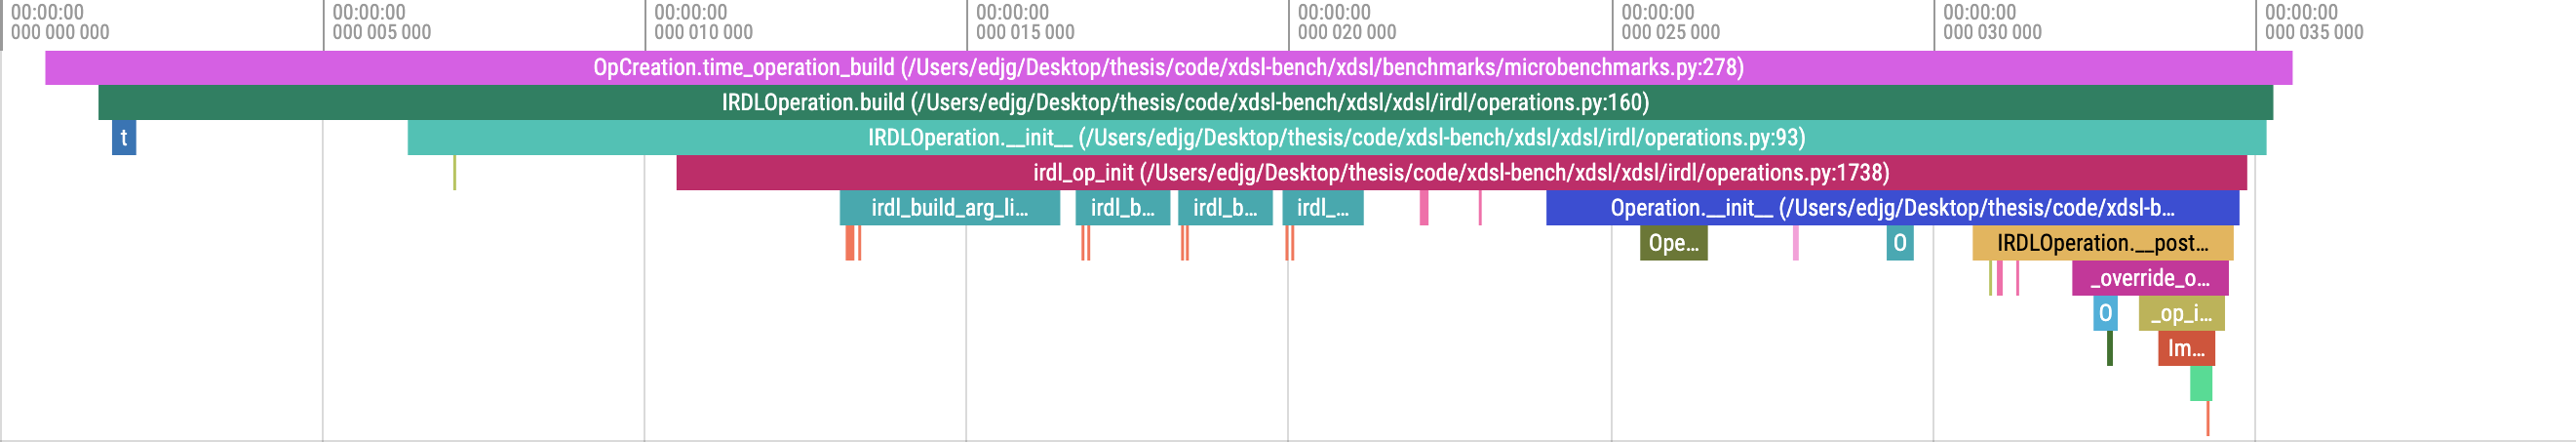
\includegraphics[width=\textwidth]{images/specialising_optimising_xdsl_rewriting/original_empty_create_scale.png}};
            \node[circledstyle, fill=pairedOneLightBlue] at (6.1,1) {A};
            \node[circledstyle, fill=pairedTwoDarkBlue] at (12.75,0.5) {B};
        \end{tikzpicture}
        \captionsetup{width=0.8\textwidth}
        \caption{The default constructor has a high overhead, calculating known invariants and .}
        \label{fig:ubenchmark-original-instantiation-xdsl-viztracer}
    \end{subfigure}
    \begin{subfigure}[b]{\textwidth}
        \centering
        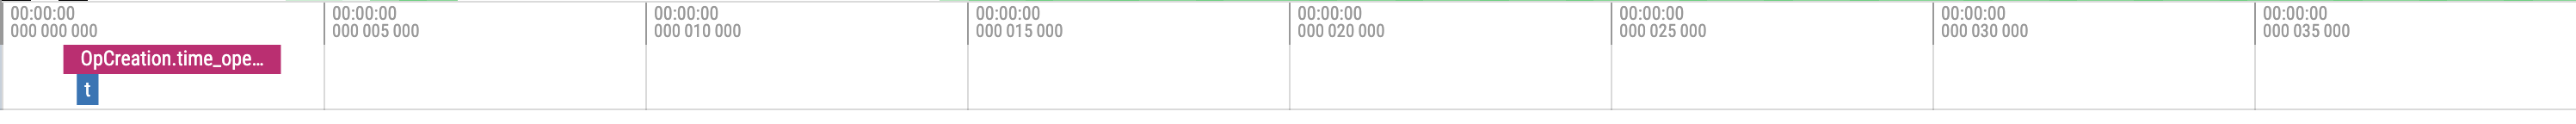
\includegraphics[width=\textwidth]{images/specialising_optimising_xdsl_rewriting/optimised_empty_create_scale.png}
        \captionsetup{width=0.8\textwidth}
        \caption{The same object can be constructed with significantly less logic.}
        \label{fig:ubenchmark-optimised-instantiation-xdsl-viztracer}
    \end{subfigure}
    \caption{\texttt{viztracer} traces of xDSL instantiating an \texttt{EmptyOp} before (top) and after (bottom) specialisation.}
    \label{fig:ubenchmark-instantiation-xdsl-viztracer}
\end{figure}

%% Describe specialisation/optimisation
% Hook
Examining the above trace, we can visually identify components which take a large proportion of runtime, and may represent unnecessary computation.
% Argument
For example, the xDSL constructor for \mintinline{python3}{IRDLOperation}s invokes logic with significant overhead building and filtering properties of the operation \circledbase{pairedOneLightBlue}{A}. However, in this workload of the empty operation, this logic does not change the constructed object. Because of this, eliding this logic results in a specialised version of the operation which generates the same output using less computation by applying domain knowledge.
In addition to this, \ac{mlir}'s core operations are not \ac{irdl} based, unlike xDSL, meaning this overhead is implementation specific.
Similarly, the post-constructor includes logic for context-managed builders \circledbase{pairedTwoDarkBlue}{B}, which is again unrelated to the empty operation case and not present in \ac{mlir}.
% Link
To avoid this overhead through specialisation, we move from the idiomatic constructor (Listing \ref{listing:ubenchmark-xdsl-constant-constructor}) to directly modifying xDSL's underlying data structures (Listing \ref{listing:ubenchmark-xdsl-constant-direct}).


\begin{figure}[H]
    \begin{subfigure}[b]{0.5\textwidth}
       \centering
        \begin{minted}[fontsize=\footnotesize]{text}
            EmptyOp()
        \end{minted}
        \caption{Instantiation with constructors.}
        \vspace{1em}
        \label{listing:ubenchmark-xdsl-constant-constructor}
    \end{subfigure}
    \hfill
    \begin{subfigure}[b]{0.5\textwidth}
        \centering
        \begin{minted}[breakanywhere,fontsize=\footnotesize]{text}
            empty_op = EmptyOp.__new__(EmptyOp)
            empty_op._operands = tuple()
            empty_op.results = tuple()
            empty_op.properties = {}
            empty_op.attributes = {}
            empty_op._successors = tuple()
            empty_op.regions = tuple()
        \end{minted}
        \caption{Instantiation by direct manipulation of xDSL's data structures.}
        \label{listing:ubenchmark-xdsl-constant-direct}
    \end{subfigure}
    \captionsetup{name=Listing}
    \caption{Approaches to instantiating an empty operation.}
    \label{listing:ubenchmark-xdsl-constant}
\end{figure}

%% Specialised performance and lessons learnt
% Hook
Through specialising the implementation to the workload of this micro-benchmark we can achieve significant performance improvements of up to $26\times$ (\autoref{tab:ubenchmark-instantiation-optimised}).
% Argument
% This process comes with the drawback of making the API much more complex
However, the performance improvement comes at the cost of a significantly more complex implementation, contrary to xDSL's design goals of a simple expressive API.
% Drop runtime by performing fewer, quicker operations
We can quantify one cause of this improvement as the specialised code executing fewer, faster bytecode instructions by leveraging our novel bytecode profiling tool (full traces in Appendices \ref{listing:bytecode-profiles-op-build-original}, \ref{listing:bytecode-profiles-op-build-optimised}).
For example, specialisation reduces the number of bytecode instructions executed from $466$ to only $29$. Function calls have a much longer duration than other instructions, with their mutation of the call stack taking up to three times longer than loading from a variable. Again leveraging our tool, we can see that specialisation reduces the number of function calls from $65$ to $5$, further contributing to the performance uplift.
By examination of its emitted bytecode (Listing \ref{listing:bytecode-profiles-op-build-optimised}), we can be confident in the optimality of the specialised implementation, as it only constructs the object and sets required fields, performing no other extraneous logic.

%% Compare performance
\begin{table}[H]
  \caption{Specialising instantiating empty operations in xDSL yields performance uplifts of up to $26\times$, only $3\times$ slower than the \ac{mlir} reference implementation.}
  \label{tab:ubenchmark-instantiation-optimised}
  \centering
  \begin{tabular}{ccc}
    \toprule
    \textbf{MLIR [ns]} & \textbf{xDSL [ns]} & \textbf{Optimised xDSL [ns]} \\
    \midrule
    $153 \pm 0.5$ & $12700 \pm 1810$ & $477 \pm 385$ \\
    \bottomrule
  \end{tabular}
\end{table}


% %% Doesn't exactly match MLIR, because dynamism means it doesn't incur heavy RTTI machinery
% % TODO: Move this into dynamism section!!!!!!!
% % Hook
% The specialised implementation achieves a slowdown of only $3\times$ from \ac{mlir}, which is surprising...
% % Argument
% % Link
% Despite this, the specialised implementation approaches the upper bound of performance for this workload as a result of the constraints of the language runtime, making it suitable for the comparison of dynamic and static language runtimes.







\subsection{Operation trait checks}
\label{ssec:specialising-ubenchmarks-trait}

%% Re-introduce microbenchmark
% Hook
The second micro-benchmark discussed involved checking traits on operations, and was measured to perform $80\times$ worse in xDSL than \ac{mlir}.
% Argument
Similarly to the operation instantiation micro-benchmark, this slow-down comes as a result of a high proportion of method's logic not being required by the core functionality (\autoref{fig:ubenchmark-hastrait-original-viztracer}). In this case, this logic improves the expressivity of the API, supporting both concrete objects and types as arguments, along with handling the edge case of unregistered operations. However, this logic lies on the hot path of execution, and again these properties are known as runtime invariants. As such, specialisation can again be leveraged to remove this implementation overhead (\autoref{fig:ubenchmark-hastrait-optimised-viztracer}).
% Link

\begin{figure}[H]
    \centering
    \begin{subfigure}[b]{\textwidth}
        \centering
        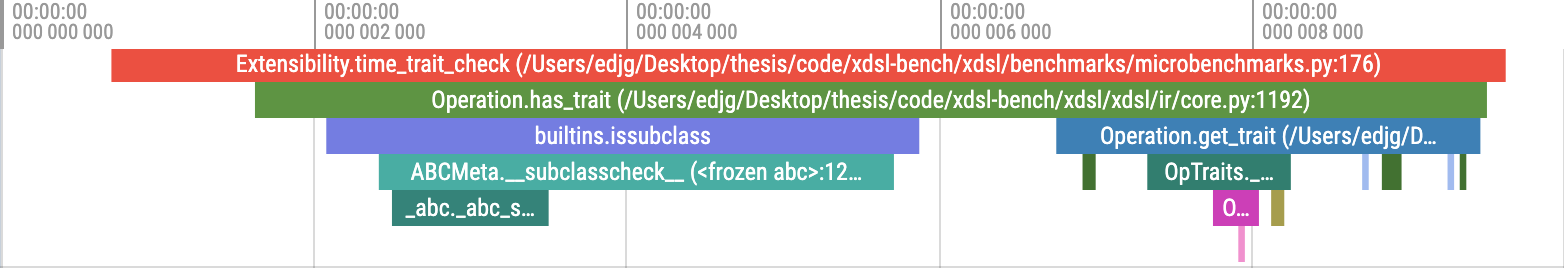
\includegraphics[width=\textwidth]{images/specialising_optimising_xdsl_rewriting/original_hastrait_scale.png}
        \captionsetup{width=0.8\textwidth}
        \caption{\mintinline{python}{issubclass} and \mintinline{python}{isinstance} checks, type \mintinline{python}{cast}ing, and constructing iterators constitutes over three quarters of xDSL's \mintinline{python}{has_trait}s runtime.}
        \label{fig:ubenchmark-hastrait-original-viztracer}
    \end{subfigure}
    \begin{subfigure}[b]{\textwidth}
        \centering
        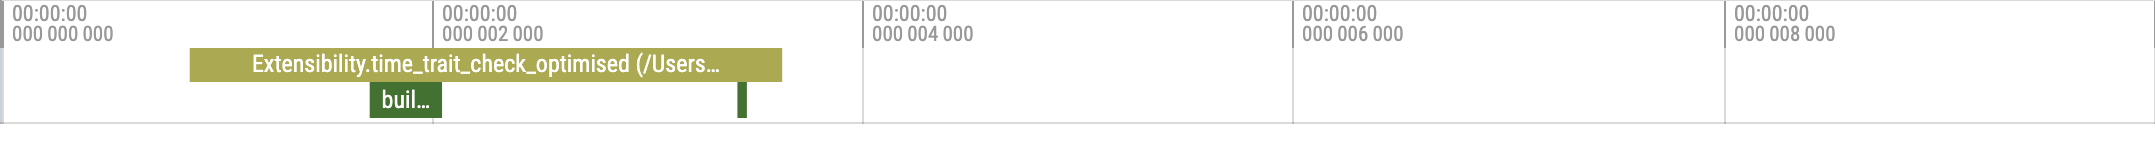
\includegraphics[width=\textwidth]{images/specialising_optimising_xdsl_rewriting/optimised_hastrait_scale.png}
        \captionsetup{width=0.8\textwidth}
        \caption{Specialisation to narrow the interface and optimisation to avoid extraneous work on hot paths can significantly accelerate \mintinline{python}{has_trait}.}
        \label{fig:ubenchmark-hastrait-optimised-viztracer}
    \end{subfigure}
    \caption{\texttt{viztracer} traces of xDSL's \mintinline{python}{has_trait} method.}
    \label{fig:ubenchmark-hastrait-viztracer}
\end{figure}

%% Describe specialisation/optimisation
% Hook
Examining the implementation of this micro-benchmark (Listing \ref{listing:ubenchmark-trait-checks-xdsl}), we can again identify opportunities for specialisation and optimisation.
% Argument
The execution trace shows that checking the whether an operation is unregistered $\circledbase{pairedOneLightBlue}{1}$ accounts for over one third of the micro-benchmark runtime. Through specialisation under the runtime invariant that all operations are registered, this check can be removed -- reducing computation. Furthermore, this inspires a general optimisation to xDSL to avoid this check by overloading \mintinline{python}{UnregisteredOp.has_trait} rather than checking on all code paths.
In addition to this, function invocation in Python incurs a performance cost due to the overhead of modifying the stack frame. As such, inlining the call to \mintinline{python}{get_trait} \circledbase{pairedTwoDarkBlue}{2} is another beneficial specialisation.
Finally, argument types are dynamically checked \circledbase{pairedThreeLightGreen}{3} and cast \circledbase{pairedFourDarkGreen}{4}, incurring a performance overhead. However, the type of these arguments are runtime invariants of the caller, so the checks can be specialised away.
% Link

\begin{figure}[H]
    \begin{subfigure}[b]{0.45\textwidth}
       \centering
        \begin{minted}[fontsize=\footnotesize,escapeinside=££]{text}
            @classmethod
            def has_trait(
                cls,
                trait: type[OpTrait] | OpTrait,
                *,
                value_if_unregistered: bool = True,
            ) -> bool:
                from xdsl.dialects.builtin import UnregisteredOp £\circledbase{pairedOneLightBlue}{\footnotesize{1}}£
                if issubclass(cls, UnregisteredOp):
                    return value_if_unregistered

                return cls.get_trait(trait) is not None £\circledbase{pairedTwoDarkBlue}{\footnotesize{2}}£
        \end{minted}
        \footnotesize\vspace{1.5em}
        \caption{Outer \mintinline{python}{has_trait} method.}
        \label{listing:ubenchmark-trait-checks-xdsl-has}
    \end{subfigure}
    \hfill
    \begin{subfigure}[b]{0.45\textwidth}
        \centering
        \begin{minted}[breakanywhere,fontsize=\footnotesize,escapeinside=££]{text}
            @classmethod
            def get_trait(
                cls,
                trait: type[OpTraitInvT] | OpTraitInvT
            ) -> OpTraitInvT | None:
                if isinstance(trait, type): £\circledbase{pairedThreeLightGreen}{\footnotesize{3}}£
                    for t in cls.traits:
                        if isinstance(t, cast( £\circledbase{pairedFourDarkGreen}{\footnotesize{4}}£
                            type[OpTraitInvT], trait
                        )):
                            return t
                else:
                    for t in cls.traits:
                        if t == trait:
                            return cast(OpTraitInvT, t)
                return None
        \end{minted}
        \caption{Inner \mintinline{python}{get_trait} method.}
        \label{listing:ubenchmark-trait-checks-xdsl-get}
    \end{subfigure}
    \vspace{1em}
    \captionsetup{name=Listing}
    \caption{xDSL methods implementing trait check functionality.}
    \label{listing:ubenchmark-trait-checks-xdsl}
\end{figure}

%% Understand specialisation
% Hook
Having specialised xDSL's implementation, we can draw direct comparison between its implementation (Listing \ref{listing:ubenchmark-trait-checks-both-xdsl}) and MLIR's (Listing \ref{listing:ubenchmark-trait-checks-both-mlir}), to better understand their relative performance characteristics.
% Argument
In contrast to the original, the specialised implementation directly matches \ac{mlir}, with the only difference being the mechanism by which traits are checked.
% Link
As such, it is well-suited for comparing the performance characteristics of static and dynamic languages independent of implementation details.

\begin{figure}[H]
    \centering
    \begin{subfigure}[b]{0.45\textwidth}
       \centering
        \begin{minted}[fontsize=\footnotesize]{text}
            for t in OP.traits._traits:
                if isinstance(t, TRAIT):
                    return True
            return False
        \end{minted}
        \footnotesize\vspace{2em}
        \captionsetup{name=Listing}
        \caption{xDSL's modified \mintinline{python}{has_trait} method.}
        \label{listing:ubenchmark-trait-checks-both-xdsl}
    \end{subfigure}
    \hfill
    \begin{subfigure}[b]{0.45\textwidth}
        \centering
        \begin{minted}[breakanywhere,fontsize=\footnotesize]{text}
            TypeID traitIDs[] = {TypeID::get<Traits>()...};
            for (unsigned i = 0, e = sizeof...(Traits); i != e; ++i)
                if (traitIDs[i] == traitID)
                    return true;
            return false;
        \end{minted}
        \captionsetup{name=Listing}
        \caption{\ac{mlir}'s \mintinline{c++}{has_trait} method.}
        \label{listing:ubenchmark-trait-checks-both-mlir}
    \end{subfigure}
    \vspace{1em}
    \captionsetup{name=Listing}
    \caption{xDSL and \ac{mlir} methods searching trait arrays.}
    \label{listing:ubenchmark-trait-checks-both}
\end{figure}

%% Specialised performance and lessons learnt
% Hook
Through specialisation, we achieve a $8\times$ speedup over the original implementation (\autoref{tab:ubenchmark-original-trait-performance}).
% Argument
However, this again incurs a cost to xDSL's expressivity, sacrificing polymorphic support for checking traits of both object types and instances. As with operation instantiation, this is contrary to xDSL's design goals.
Furthermore, this speedup is less dramatic than operation instantiation, as a result of having less overhead in the original implementation, but can be reasoned about in the same manner with our novel profiling tool (full traces in Appendices \ref{listing:bytecode-profiles-hastrait-original}, \ref{listing:bytecode-profiles-hastrait-optimised}). As before, specialisation reduces the number of bytecode instructions from $89$ to $35$, with the number of high-overhead \texttt{CALL} instructions dropping from $11$ to $2$.
% Link
% In addition to this, the similarity of the two implementations allows us to draw comparisons between the bytecode and assembly instructions.

% %% Compare performance and number of bytecode/assembly operations
% \begin{figure}[H]
%     \centering
%     \begin{subfigure}[b]{0.45\textwidth}
%         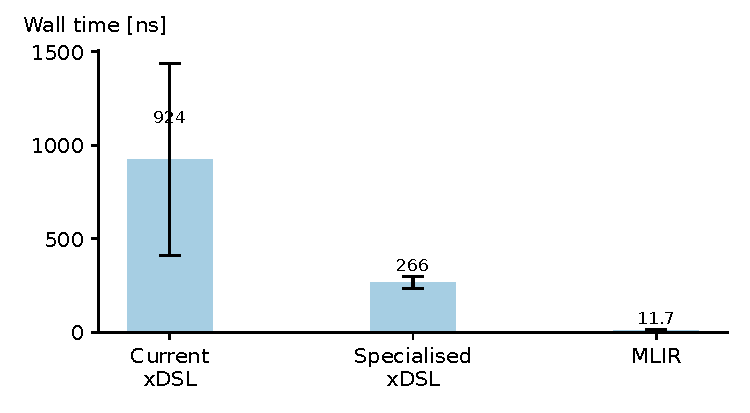
\includegraphics[width=\textwidth]{images/specialising_optimising_xdsl_rewriting/trait_performance.pdf}
%         \caption{Specialisation yields performance uplifts of up to $3.5\times$, $23\times$ slower than the \ac{mlir} reference implementation.}
%         \label{fig:ubenchmark-original-trait-performance}
%         \vspace{1em}
%     \end{subfigure}
%     \hfill
%     \begin{subfigure}[b]{0.45\textwidth}
%         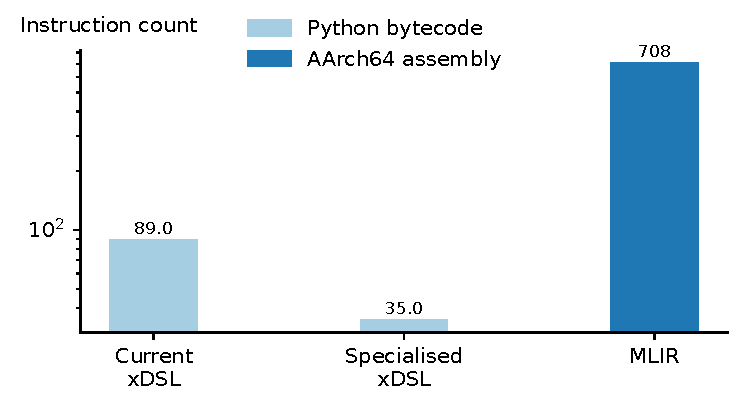
\includegraphics[width=\textwidth]{images/specialising_optimising_xdsl_rewriting/trait_instructions.pdf}
%         \caption{Specialisation reduces the bytecode instruction count by $2.5\times$, with complex Python bytecode instructions expressing more functionality than RISC AArch64 assembly.}
%         \label{fig:ubenchmark-original-trait-instructions}
%     \end{subfigure}
%     \caption{Impact of specialising trait checking xDSL on performance and instruction count.}
%     \label{fig:ubenchmark-original-trait-summary}
% \end{figure}

\begin{table}[H]
  \caption{specialising trait checking in xDSL yields performance uplifts of up to $8\times$, $20\times$ slower than the \ac{mlir} reference implementation.}
  \label{tab:ubenchmark-original-trait-performance}
  \centering
  \begin{tabular}{ccc}
    \toprule
    \textbf{MLIR [ns]} & \textbf{xDSL [ns]} & \textbf{Optimised xDSL [ns]} \\
    \midrule
    $11.7 \pm 0.5$ & $1920 \pm 695$ & $239 \pm 35$ \\
    \bottomrule
  \end{tabular}
\end{table}

% % TODO: Does this want to be lifted into the dynamism section -- this might make it easier to link to more substantial data rather than just explaining interpreter/compiler again in gratuitous detail
% % Hook
% Empowered by the similarity of their implementations, we can further apply profiling tools to contrast the emitted instructions by each language runtime.
% % Argument
% For xDSL's Python, we use our novel bytecode profiling tool ByteSight, and for \ac{mlir}'s C++, we use \texttt{valgrind}'s \texttt{callgrind} tool \cite{valgrindtmdevelopersCallgrindCallgraphGenerating}.
% For the same algorithm, Python dispatches only $35$ bytecode instructions in comparison with AArch64 assembly taking $708$ (\autoref{fig:ubenchmark-original-trait-performance}).
% This demonstrates the significant abstraction gap between high-level Python bytecode and the low-level assembly instructions compiled from C++. While Python requires fewer explicit instructions due to its dynamic dispatch and built-in operations handling complex tasks internally, the underlying C++ implementation must execute many more granular assembly instructions to achieve the same computational result.
% % Link
% Despite this, the C++ implementation outperforms the Python implementation, due to these assembly instructions more closely matching the execution model of the target machine.







%% ======================================================== %%
%% This subsection would just repeat the points made above? %%
%% ======================================================== %%
% \subsection{What does specialisation do?}
% \label{ssec:specialising-what-do}
% %% What does specialisation do
% % Hook
% From the above two micro-benchmarks, we have empirically demonstrated that specialisation to workloads improves their performance, approaching the best-case .
% % Argument
% The mechanism for this is simple: specialisation uses extra information in the form of runtime invariants to avoid work at runtime, reducing the number of bytecode instructions the interpreter needs to execute.
% % Relate into JIT compilation and stuff
% % Link
% Having demonstrated and understood the effectiveness of specialisation for small workloads, we can now leverage it for a non-trivial example of pattern rewriting.
%% Summary table??
% \begin{table}[H]
% %   \caption{Specialisation improves xDSL's operation instantiation performance by $26\times$, lifting it from $83\times$ to $3\times$ slower than \ac{mlir}.}
%   \caption{Specialisation improves xDSL's performance for micro-benchmarks.}
%   \label{tab:ubenchmark-instantiation-optimised}
%   \centering
%   \begin{tabular}{cccc}
%     \toprule
%     \textbf{} & \textbf{MLIR [ns]} & \textbf{xDSL [ns]} & \textbf{Specialised xDSL [ns]} \\
%     \midrule
%     Operation instantiation & $153 \pm 0.5$ & $12700 \pm 1810$ & $477 \pm 385$ \\
%     % Operation instantiation & $357 \pm 0.5$ & $33400 \pm 3680$ & $1830 \pm 774$ \\
%     Trait checking & $11.7 \pm 0.5$ & $924 \pm 513$ & $266 \pm 34$\\
%     \bottomrule
%   \end{tabular}
% \end{table}







\section{Pattern rewriting}
\label{sec:specialising-pattern-rewriting}

%% Introduce actual workload over micro-benchmarks
% Hook
Having demonstrated specialisation as an approach to examine the performance bound of a language runtime for micro-benchmarks, we can further apply it to real-world workloads such as constant folding.
% Argument
In this section, we specialise a simple pattern rewriter: constant folding over integer addition.
% Unlike previous micro-benchmarks, MLIR's implementation of pattern rewriting also introduces non-negligible implementation overhead. As such, we provide a matching implementation of this algorithm in MLIR to guarantee fair comparison.
% Link
These specialised implementations can then be taken as performance baselines for their respective languages, and further analysed through bytecode tracing or disassembly to understand their implementation.


\subsection{Constant folding}
\label{sec:specialising-pattern-rewriting-workload}

%% Summarise the workload and how it is special
% Hook
For our first benchmarks of the two frameworks, we measured the end-to-end performance of canonicalization passes applied to an \ac{ir} with many foldable constants (\autoref{sssec:experimental-workload-constant-folding}).
% Argument
However, canonicalization passes are fairly complex, encompassing a suite of common optimisations, many of which are not applicable to our \ac{ir} workload. This complexity is detrimental to manual specialisation, resulting in more code requiring transformation by hand.
As such, we implement a simple pattern rewriting pass for constant folding over the addition of integers (\autoref{listing:constant-folding-impl}). This pass captures common idioms in pattern rewriting, making it a fair proxy for more complex workloads, but is also sufficiently simple to rewrite by hand into a fully specialised form.
The rewriter first matches against the integer addition operation to fold \circledbase{pairedOneLightBlue}{1}, exercising operation type checks. Next, it checks the invariant of our workload that both addition operands are constant \circledbase{pairedTwoDarkBlue}{\scriptsize{2}}, exercising trait lookups. After this, it gets the value of each operand, exercising operation properties \circledbase{pairedThreeLightGreen}{\scriptsize{3}}. Finally, it replaces the matched operation with a new one, exercising the rewriting mechanism \circledbase{pairedFourDarkGreen}{\scriptsize{4}}.
% Link   % TODO: Think of some link

%% Listing showing the two implementations
\begin{figure}[H]
    \centering
    \begin{subfigure}[b]{0.45\textwidth}
       \centering
        \begin{minted}[fontsize=\scriptsize,escapeinside=££]{text}
def match_and_rewrite(self, op: Operation, rewriter: PatternRewriter, /):
    # Only rewrite integer add operations £\circledbase{pairedOneLightBlue}{\scriptsize{1}}£
    if not isinstance(op, AddiOp):
        return

    # Ensure both operands are constants £\circledbase{pairedTwoDarkBlue}{\scriptsize{2}}£
    lhs_op = op.operands[0].op
    rhs_op = op.operands[1].op
    assert lhs_op.has_trait(ConstantLike)
    assert rhs_op.has_trait(ConstantLike)

    # Calculate the result of the addition £\circledbase{pairedThreeLightGreen}{\scriptsize{3}}£
    lhs = lhs_op.value.value.data
    rhs = rhs_op.value.value.data
    folded_op = ConstantOp(
        IntegerAttr(lhs + rhs, op.result.type)
    )

    # Rewrite with the calculated result £\circledbase{pairedFourDarkGreen}{\scriptsize{4}}£
    rewriter.replace_matched_op(
        folded_op, [folded_op.results[0]]
    )
        \end{minted}
        \footnotesize\vspace{5em}
        \captionsetup{name=Listing}
        \caption{xDSL implementation.}
        \label{listing:constant-folding-impl-xdsl}
    \end{subfigure}
    \hfill
    \begin{subfigure}[b]{0.5\textwidth}
        \centering
        \begin{minted}[breakanywhere,fontsize=\scriptsize,escapeinside=££]{text}
  // Only rewrite integer add operations £\circledbase{pairedOneLightBlue}{\scriptsize{1}}£
  LogicalResult matchAndRewrite(arith::AddIOp op, PatternRewriter &rewriter) const override {

    // Ensure both operands are constants £\circledbase{pairedTwoDarkBlue}{\scriptsize{2}}£
    arith::ConstantOp lhsConstOp = op.getLhs().getDefiningOp<arith::ConstantOp>();
    arith::ConstantOp rhsConstOp = op.getRhs().getDefiningOp<arith::ConstantOp>();
    if (!lhsConstOp || !rhsConstOp) {
        return failure();
    }

    // Calculate the result of the addition £\circledbase{pairedThreeLightGreen}{\scriptsize{3}}£
    auto lhsAttr = lhsConstOp.getValue().dyn_cast<IntegerAttr>();
    auto rhsAttr = rhsConstOp.getValue().dyn_cast<IntegerAttr>();
    if (!lhsAttr || !rhsAttr) {
        return failure();
    }
    APInt lhsValue = lhsAttr.getValue();
    APInt rhsValue = rhsAttr.getValue();
    APInt result = lhsAttr.getValue() + rhsAttr.getValue();

    // Rewrite with the calculated result £\circledbase{pairedFourDarkGreen}{\scriptsize{4}}£
    auto resultType = op.getType();
    auto foldedValue = rewriter.getIntegerAttr(resultType, result);
    rewriter.replaceOpWithNewOp<arith::ConstantOp>(op, resultType, foldedValue);
    return success();
  }
        \end{minted}
        \captionsetup{name=Listing}
        \caption{\ac{mlir} implementation.}
        \label{listing:constant-folding-impl-mlir}
    \end{subfigure}
    \vspace{1em}
    \captionsetup{name=Listing}
    \caption{Implementations of pattern rewriters for constant folding over integer addition.}
    \label{listing:constant-folding-impl}
\end{figure}

%% Implementation details and why separate xDSL and MLIR?
% Hook
In order to draw fair comparisons between the two frameworks, their implementations of the constant folding pattern rewrite must be equivalent.
% Argument
As such, we provide implementations for both xDSL (Listing \ref{listing:constant-folding-impl-xdsl}) and \ac{mlir} (Listing \ref{listing:constant-folding-impl-xdsl}).
Measuring the \ac{mlir} implementation is complicated by the fact that its pattern rewriting infrastructure implements constant folding by default. To mitigate this, we manually excise this functionality from the \ac{mlir} framework to ensure that our pattern rewriting kernel is the implementation being measured.
% Link
Having constructed these implementations, we can follow the same specialisation process introduced for the micro-benchmarks to bring the xDSL's performance closer to the best-case for that workload in the Python language.
% Unlike previous micro-benchmarks, MLIR's implementation of pattern rewriting also introduces non-negligible implementation overhead. As such, we provide a matching implementation of this algorithm in MLIR to guarantee fair comparison.
% In addition to this, unlike previous micro-benchmarks, MLIR's implementation of pattern rewriting introduces significant overhead by providing expressivity in the form of features such as rewriting callbacks.


\subsection{Specialisation}
\label{sec:specialising-pattern-rewriting-specialisation}

%% What does specialisation mean in this context (inlining/eliding/...)
% Link
Although our constant folding pass is less intricate than existing passes such as canonicalisation, it is still much more complex than any of the above micro-benchmarks (\autoref{fig:constant-fold-original-viztracer}).
% As such, there are many more opportunities for the specialisation of its implementation.
% Argument
Instead of one or two helper functions in xDSL's API, aspects of the pattern rewriter such as replacing the matched operation have a deep call stack, invoking methods to set many aspects of the \ac{ir}'s object representation.
As such, the first step in the specialisation process is manually inlining this call stack, which provides two benefits. Firstly, it avoids the non-negligible overhead of function calls discussed in previous micro-benchmarks, and further worsened by the deep call stack of the more complex implementation. Secondly, it reveals logic that is redundant for the implementation of this workload, which is otherwise hidden across the boundaries of xDSL's API.
The inlined implementation can then be specialised to remove this redundant logic, and further leverage runtime invariants of the integer constant addition workload where possible.
% Link
This yields a specialised implementation with reduced overhead (\autoref{fig:constant-fold-optimised-viztracer}).


\begin{figure}[H]
    \centering
    \begin{subfigure}[b]{\textwidth}
        \centering
        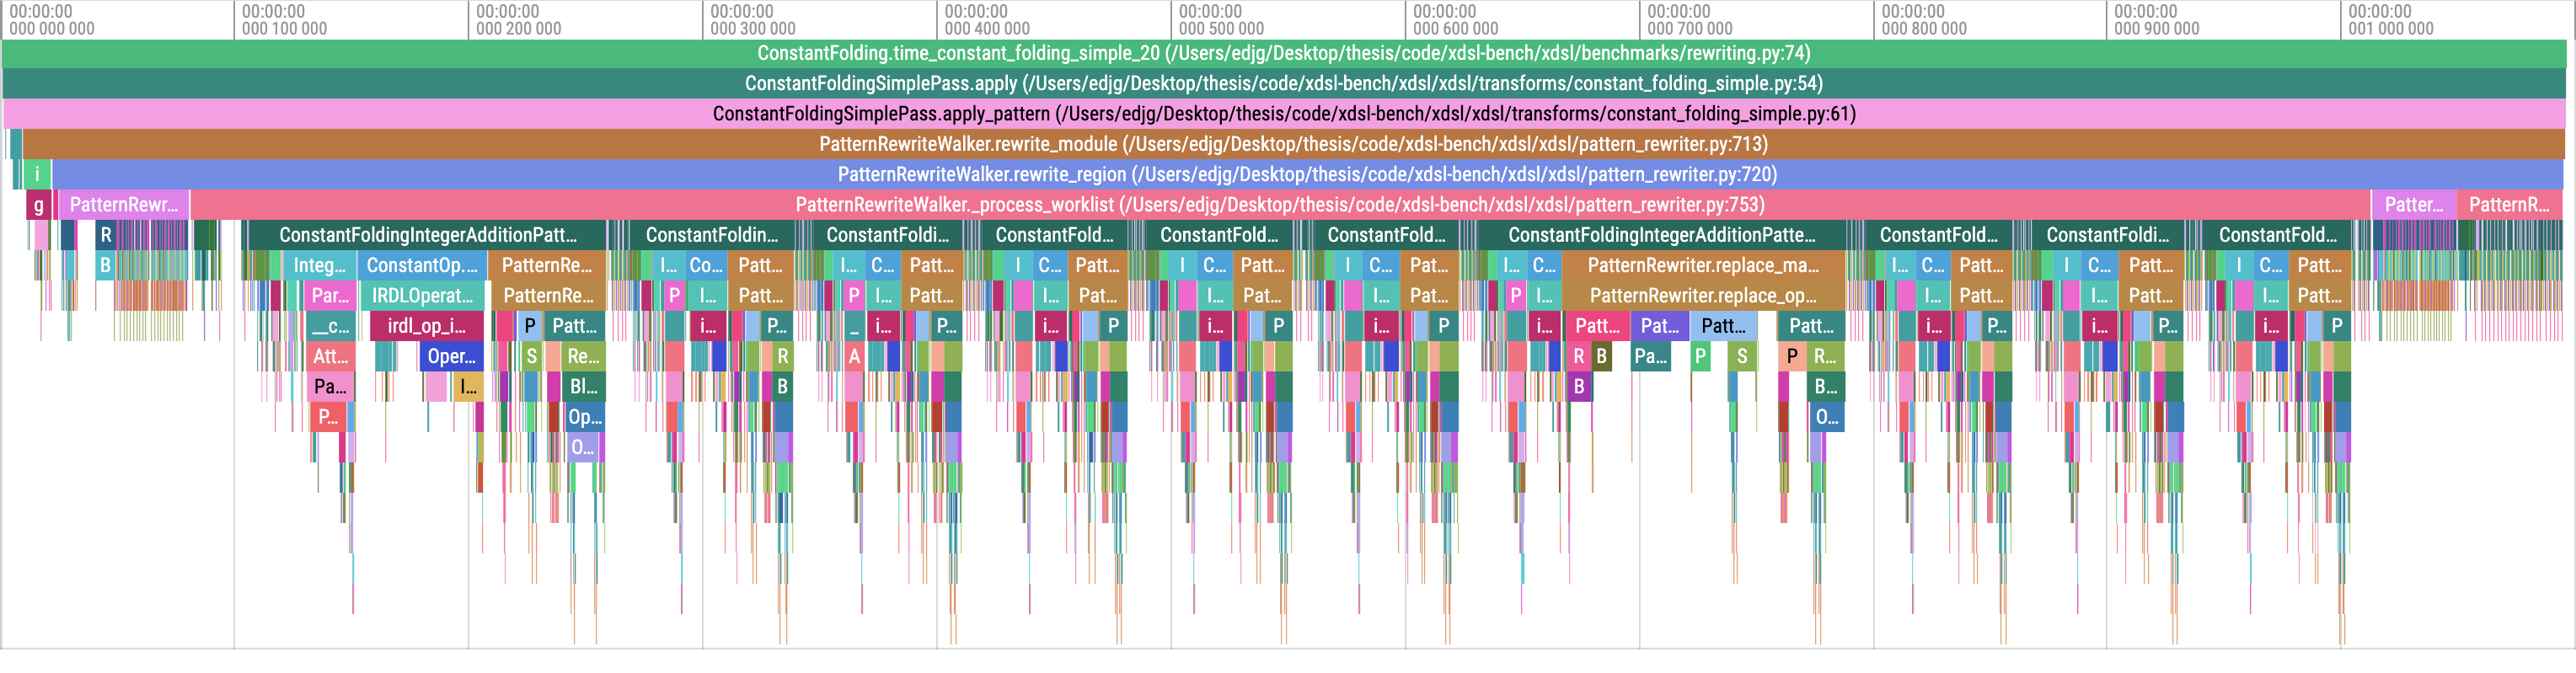
\includegraphics[width=\textwidth]{images/specialising_optimising_xdsl_rewriting/custom_constant_fold_scale.png}
        \captionsetup{width=0.8\textwidth}
        \caption{xDSL's existing pattern rewriting infrastructure has a high performance overhead, executing many extraneous operations with a deep call stack.}
        \label{fig:constant-fold-original-viztracer}
    \end{subfigure}
    \begin{subfigure}[b]{\textwidth}
        \centering
        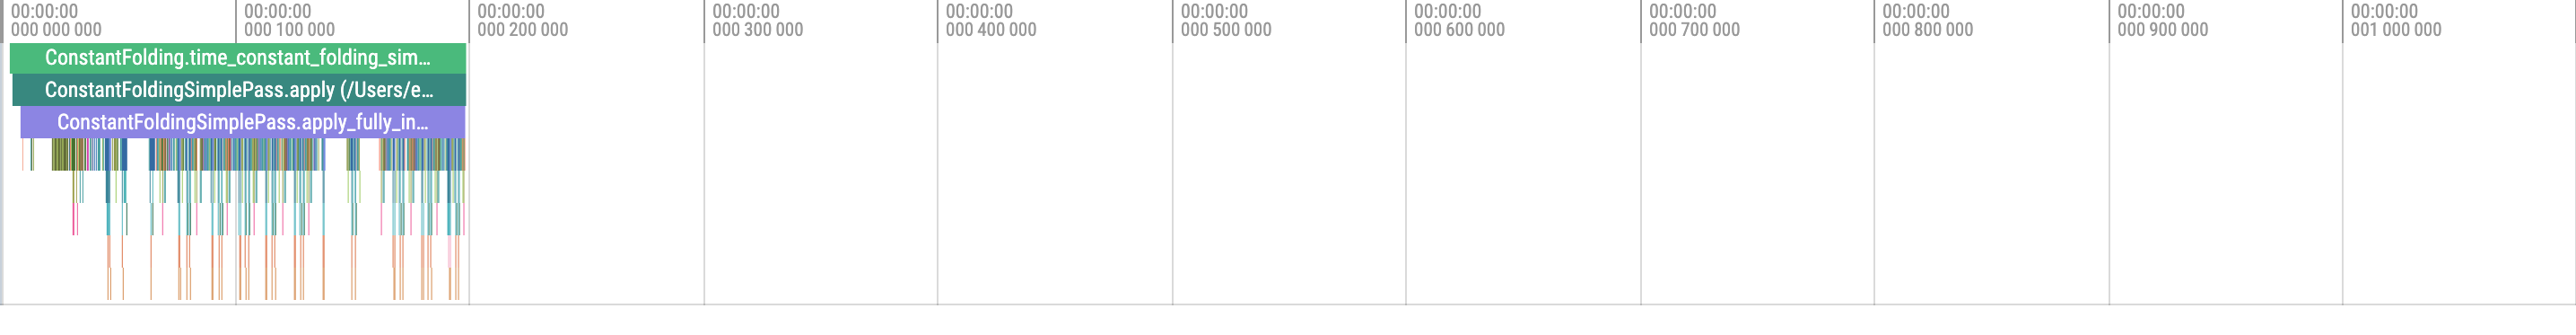
\includegraphics[width=\textwidth]{images/specialising_optimising_xdsl_rewriting/optimised_constant_fold_scale.png}
        \captionsetup{width=0.8\textwidth}
        \caption{Through specialisation, this overhead can be significantly reduced, performing the exact workload and only invoking inbuilt functions such as set operations and \mintinline{python}{isinstance} checks.}
        \label{fig:constant-fold-optimised-viztracer}
    \end{subfigure}
    \caption{\texttt{viztracer} traces of xDSL's integer addition constant folding pattern rewrite.}
    \label{fig:constant-fold-viztracer}
\end{figure}


\subsection{Performance improvement}
\label{sec:specialising-pattern-rewriting-performance}

%% How much did we get/lose out of this?
% Link
Through specialising the constant folding implemenation, we achieve a $8\times$ speedup over the original implementation (\autoref{fig:constant-fold-summary}).
% Argument
However, this performance uplift comes at the cost of ease of implementation, increasing the constant folding implementation length by $7\times$ (\autoref{fig:constant-fold-loc}).
As with the specialised micro-benchmarks, we can leverage our novel bytecode profiling tool to explain this improvement in terms of dispatched bytecode instructions, with the workload dropping from $5465$ to $977$ instructions required to implement its functionality.
By examining the implementation and its emitted bytecode instructions, we are confident that it is close to optimal for the workload within the context of xDSL's data structures.
In combination with the modifications made to \ac{mlir} to similarly avoid extraneous computation, these two implementations are both directly comparable and complex enough to be representative of real-world workloads.
% Link
This facilitates their later use for exploring the impact of dynamism on such workloads.



% TODO? Further weaknesses of workload so large hard to reason about and MLIR itself has implementation details adding overhead -- but does demonstrate xDSL can be improved and lower bound C++ performance

%% Figure or table comparing performance
\begin{figure}[H]
    \centering
    \begin{subfigure}[b]{0.45\textwidth}
        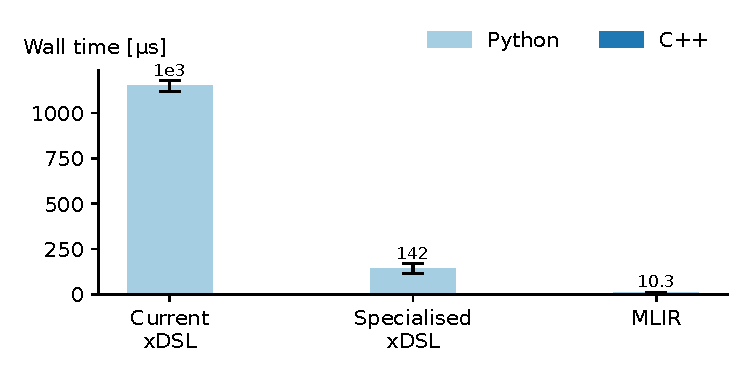
\includegraphics[width=\textwidth]{images/specialising_optimising_xdsl_rewriting/constant_performance.pdf}
        \caption{Specialisation yields performance uplifts of
up to $8\times$, $14\times$ slower than the MLIR reference
implementation.}
        \label{fig:constant-fold-performance}
        % \vspace{1em}
    \end{subfigure}
    \hfill
    \begin{subfigure}[b]{0.45\textwidth}
        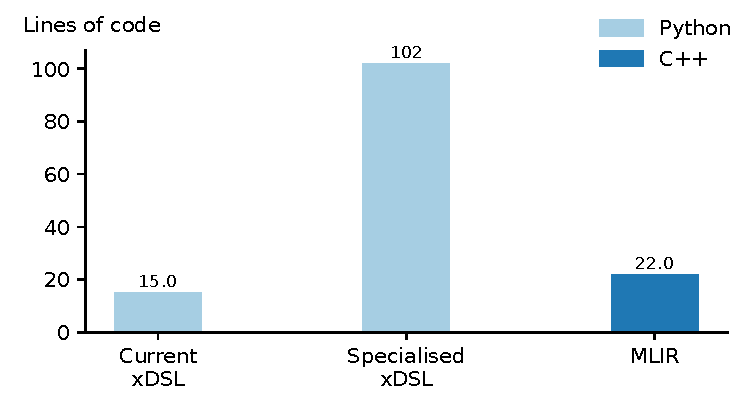
\includegraphics[width=\textwidth]{images/specialising_optimising_xdsl_rewriting/constant_loc.pdf}
        \caption{Specialisation increases the implementation length of the rewriter by $7\times$.} % TODO: Could also add cognitive complexity?
        \label{fig:constant-fold-loc}
        \vspace{1em}
%         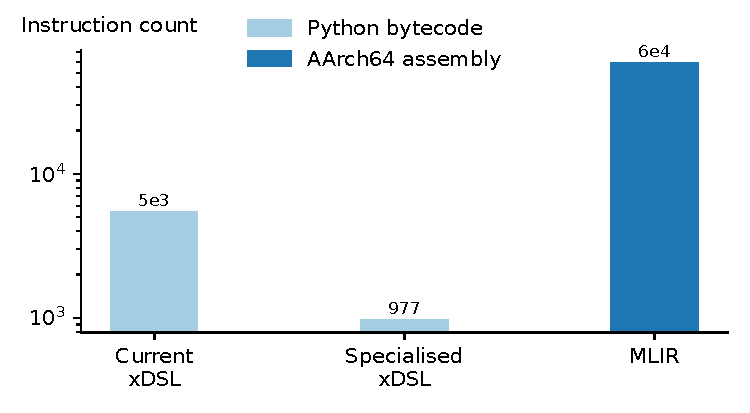
\includegraphics[width=\textwidth]{images/specialising_optimising_xdsl_rewriting/constant_instructions.pdf}
%         \caption{Specialisation reduces the bytecode instruc-
% tion count by $5.5\times$, with complex Python byte-
% code instructions expressing more functionality
% than RISC AArch64 assembly.}
%         \label{fig:constant-fold-instructions}
    \end{subfigure}
    \caption{Impact of specialising constant folding of integer addition in xDSL on performance and implementation length.}
    % \caption{Impact of specialising constant folding of integer addition in xDSL on performance and instruction count.}
    \label{fig:constant-fold-summary}
\end{figure}
% \begin{table}[H]
%   \caption{.}
%   \label{tab:constant-folding-optimised}
%   \centering
%   \begin{tabular}{ccc}
%     \toprule
%     \textbf{MLIR [$\bm{\mu}$s]} & \textbf{xDSL [$\bm{\mu}$s]} & \textbf{Optimised xDSL [$\bm{\mu}$s]} \\
%     \midrule
%     $10.3 \pm 0.1$ & $1150 \pm 30$ & $142 \pm 30$\\
%     \bottomrule
%   \end{tabular}
% \end{table}
% Test ConstantFoldingSimple.20(unspecialised) ran in: 0.00115 ± 3e-05s
% Test ConstantFoldingSimple.20(specialised) ran in: 0.000142 ± 2.92e-05s
% SimpleConstantFolding/folding/1          10112 ns        10070 ns        70189
% SimpleConstantFolding/folding/8          81970 ns        81663 ns         8557
% SimpleConstantFolding/folding/64        640847 ns       638256 ns         1074
% SimpleConstantFolding/folding/512      5222675 ns      5202763 ns          135
% SimpleConstantFolding/folding/4096    42047737 ns     41843492 ns           17
% SimpleConstantFolding/folding/10000  100531426 ns    100120405 ns            7
% SimpleConstantFolding/folding_BigO    10083.92 N      10041.57 N
% SimpleConstantFolding/folding_RMS            1 %             1 %

% 58594 events in
% mlir::applyPatternsAndFoldGreedily(mlir::Region&, mlir::FrozenRewritePatternSet const&, mlir::GreedyRewriteConfig, bool*)



\subsection{Optimisations}
\label{sec:specialising-pattern-rewriting-optimisations}

%% Introduction + scope of stuff
% Hook
The majority of changes made during specialisation are applicable only to their specific workload.
% Argument
However, some are more generic to any use case of xDSL, and as such can be applied as stand-alone optimisations. Unfortunately, xDSL is a large codebase, over $150,000$ lines of Python, and as such it is out of scope of this thesis to improve the performance of all of it.
Despite this, we demonstrate that the specialisation process lead to generalisable optimisations with measurable performance impact.
Through this, we enable performance improvement over time, which can be quantified using our previously introduced measurement infrastructure (\autoref{ssec:infrastructure}).
% Link
In this section, we discuss two salient examples of the generalised optimisations.

%% Removing overhead in functions
% Link
During the specialisation process of trait checking (\autoref{ssec:specialising-ubenchmarks-trait}), we saw that the implementation of xDSL's \texttt{has\_trait} helper function introduces significant overhead by checking the infrequent case of unregistered operations on the hot path of execution.
% Argument
Since this functionality was not used by the target workload, this could be elided by specialisation for performance. However, it also reveals an optimisation which can be applied to the general case:
% Link
This optimisation was applied in \href{https://github.com/xdslproject/xdsl/pull/4242}{PR \#4242}, resulting in a $2.1\times$ speedup on micro-benchmarks and $1.15\times$ speedup within the specialised constant folding workload. % Effect becomes dominated by noise for unspecialised constant folding, which takes an order of magnitude longer.

%% Removing implicit builders
% Link
Similarly, the specialisation of operation instantiation (\autoref{ssec:specialising-ubenchmarks-instantiation}) revealed the performance impact of managing the scope of implicit builders, even when they are not being used.
% Argument
As before, this can be generalised to change xDSL's approach from always invoking logic to handle implicit builders irrespective of whether they are used, to only for operation instantiations which use them.
% Link
This optimisation was applied in \href{https://github.com/xdslproject/xdsl/pull/4163}{PR \#4163}, resulting in a $1.06\times$ speedup on micro-benchmarks and $1.01\times$ speedup within the specialised constant folding workload. % Effect becomes dominated by noise for unspecialised constant folding, which takes an order of magnitude longer.


%% Optional stretch goal to be filled in later...?
%% `__slots__` (stretch dataclasses stuff -> custom dataclass like thing without most of the overhead as a helper, replaces frozen dataclasses (what functionality is used here: https://github.com/python/cpython/blob/main/Lib/dataclasses.py and what can we rip out???))


\section{Summary}
\label{sec:specialising-summary}


%% Final performance figures
% Hook
Through empirical measurement, we approach the best-case performance of Python for pattern rewriting in user-extensible compiler infrastructure.
% Argument
We demonstrate that specialised Python implementations of real-world pattern rewriting workloads can improve xDSL's performance by $8\times$, to be only $14\times$ slower than the equivalent \ac{mlir} implementation. This specialisation avoids computation which is redundant for the selected workload, and avoids costs associated with function invocation.
% In addition to this, for some workloads we find that Python's performance can further approach C++,
We further show that this specialisation process reveals optimisations that can be generalised to improve xDSL beyond the individual workload.
%
In the next chapters, we leverage this best-case performance specialisation as a baseline to examine the effect of both recent improvements to CPython's runtime, and the cost of dynamism in comparison with statcially compiled languages.
